\chapter{Distances on directed graphs}
\label{cha:dist-direct-graphs}
We discussed in this chapter the extensions of some of the notions of
distances on undirected graphs in Chapter \ref{cha:dist-undir-graphs}
to directed graphs. We concern ourselves mainly with the notions of
expected commute times, diffusion distances, and forest metrics. 
\section{Expected commute time for directed graphs}
\label{sec:expect-comm-time-1}
The notion of expected commute time as defined in
Eq. \eqref{eq:25} extends naturally onto directed graphs. Let $G =
(V,E,\omega)$ be a directed graph with similarity measure
$\omega$. Let $\mathbf{P}$ be the transition matrix of the random walk
on $G$ defined as in \S \ref{sec:random-walks-graphs}. 
If $\mathbf{M}$ is the matrix of mean first passage time with respect
to $\mathbf{P}$, then $\mathbf{M}$ also satisfies the matrix equation
(see Proposition \ref{prop:4}). 
\begin{equation*}
   (\mathbf{I} - \mathbf{P})\mathbf{X} = \mathbf{J} - \bm{\Pi}^{-1}
\end{equation*}
subjected to the condition 
\begin{equation*}
 \mathbf{M}_{\mathrm{dg}} = \mathbf{0}, \qquad \mathbf{M}(u,v) \geq 0   
\end{equation*}
$\mathbf{M}$ is again given by
Eq. \eqref{eq:21}. $\Delta_{\delta}$, the matrix of expected commute
time, is then given by
\begin{equation}
  \label{eq:73}
  \begin{split}
    \Delta_\delta &= \mathbf{J}(\mathbf{Z}\bm{\Pi}^{-1})_{\mathrm{dg}}
    - \mathbf{Z}\bm{\Pi}^{-1} - \bm{\Pi}^{-1}\mathbf{Z}^{T} +
    (\bm{\Pi}^{-1}\mathbf{Z})_{\mathrm{dg}}\mathbf{J} \\ \ &=
    \tfrac{1}{2}\kappa(\mathbf{Z}\bm{\Pi}^{-1} +
    \mathbf{\Pi}^{-1}\mathbf{Z}^{T})
  \end{split}
\end{equation}
%
The following result established that $\Delta_{\delta}$ for directed
graphs is also EDM-2.
\begin{proposition}
  \label{prop:19}
 $\mathbf{Z}\bm{\Pi}^{-1} + \bm{\Pi}^{-1}\mathbf{Z}^{T}$ is
 positive definite. By Proposition \ref{prop:18},
 $\Delta_{\delta}$ is EDM-2.  
\end{proposition}
\begin{proof}
  We use the
  following characterizations of positive definite matrices
  \citep[see][\S
  1.2]{boley09:_gener_laplac,horn94:_topic_in_matrix_analy}. If
  $\mathbf{A}$ is invertible, then
  \begin{equation}
    \label{eq:74}
    \mathbf{A} + \mathbf{A}^{T} \succ 0 \Leftrightarrow
    \mathbf{A}^{-1} + (\mathbf{A}^{-1})^{T} \succ 0
  \end{equation}
  Since $\mathbf{Z}\bm{\Pi}^{-1}$, we have
  \begin{equation}
    \label{eq:75}
    \begin{split}
   \mathbf{Z}\bm{\Pi}^{-1} + \bm{\Pi}^{-1}\mathbf{Z}^{T} \succ 0
   & \Leftrightarrow \bm{\Pi}(\mathbf{I} - \mathbf{P} + \mathbf{Q}) +
   (\mathbf{I} - \mathbf{P}^{T} + \mathbf{Q}^{T}) \bm{\Pi} \succ 0  \\
   & \Leftrightarrow \bm{\Pi}(\mathbf{I} - \mathbf{P}) +
   \bm{\Pi}(\mathbf{I} - \hat{\mathbf{P}}) + 2 \pi \pi^{T} \succ 0 \\
   & \Leftrightarrow 2 \bm{\Pi}\Bigl(\mathbf{I} - \frac{\mathbf{P} +
     \hat{\mathbf{P}}}{2}\Bigr) + 2\pi\pi^{T} \succ 0
   \end{split}
  \end{equation}
  where $\hat{\mathbf{P}}$ is the time-reversal of $\mathbf{P}$. Since
  $\hat{\mathbf{P}}$ is also a stochastic matrix,
  $\bm{\Pi}\Bigl(\mathbf{I} - \tfrac{\mathbf{P} +
    \hat{\mathbf{P}}}{2}\Bigr)$ is symmetric and diagonally dominant. Thus
  $\bm{\Pi}\Bigl(\mathbf{I} - \tfrac{\mathbf{P} +
    \hat{\mathbf{P}}}{2}\Bigr) \succeq 0$. This implies that
  $\mathbf{Z}\bm{\Pi}^{-1} + \bm{\Pi}^{-1}\mathbf{Z}^{T}$ is positive
  definite. 
\end{proof}
Some observations about expected commute time for directed graphs can
be made by representing $\mathbf{Z}\bm{\Pi}^{-1} +
\bm{\Pi}^{-1}\mathbf{Z}^{T}$ as a power series. We know from \S
\ref{sec:expect-comm-time} that $\mathbf{Z}\bm{\Pi}^{-1}$ has the
series expansion
\begin{equation*}
  \mathbf{Z}\bm{\Pi}^{-1} = \Bigl[ \mathbf{I} +
  \sum_{k=1}^{\infty}(\mathbf{P}^{k} - \mathbf{Q})\Bigr] \bm{\Pi}^{-1}
\end{equation*}
From Eq.~\eqref{eq:78} and the fact that $\mathbf{Q}\bm{\Pi}^{-1} =
\mathbf{J}$, we therefore have 
\begin{equation*}
  \begin{split}
\bm{\Pi}^{-1} \mathbf{Z}^{T} &= \bm{\Pi}^{-1} \Bigl[ \mathbf{I} +
  \sum_{k=1}^{\infty}((\mathbf{P}^{k})^{T} - \mathbf{Q}^{T})\Bigr] \\
  &= \Bigl[ \mathbf{I} +
  \sum_{k=1}^{\infty}(\hat{\mathbf{P}}^{k} - \mathbf{Q})\Bigr]
  \bm{\Pi}^{-1}
  \end{split}
\end{equation*}
The series expansion for $\mathbf{Z}\bm{\Pi}^{-1} +
\bm{\Pi}^{-1}\mathbf{Z}^{T}$ is then given by
\begin{equation}
  \label{eq:80}
  \mathbf{Z}\bm{\Pi}^{-1} + \bm{\Pi}^{-1}\mathbf{Z}^{T} = 
 2 \Bigl[ \mathbf{I} +
  \sum_{k=1}^{\infty}\Bigl(\frac{\mathbf{P}^{k} + \hat{\mathbf{P}}^{k}}{2}
  - \mathbf{Q}\Bigr)\Bigr] \bm{\Pi}^{-1}
\end{equation}
Eq.~\eqref{eq:80} states that expected commute time between $u$ and
$v$ is composed of two parts that are basically time-reversal of each
other. This is consistent with the observation that $\mathbf{M}(u,v)$,
the mean first passage time from $u$ to $v$, can be obtained from the
time-reversal random walk starting from $v$ going back to
$u$. Eq.~\eqref{eq:80} also indicates that the symmetrization in
expected commute time for a directed graph $G$ is performed at a later
stage than that obtained by viewing $G$ as an undirected
graph. Finally, we can also view Eq.~\eqref{eq:80} as being a special
case of combining similarities from multiple graphs $G_k$, with each
graph $G_k$ having $\bm{\Pi}(\mathbf{P}^{k} + \hat{\mathbf{P}}^{k})$
as its similarity matrix.
\section{Diffusion distances for directed graphs}
\label{sec:diff-dist-direct}
The starting point for the definition of diffusion distances for
directed graphs is Eq.~\eqref{eq:43}, which we recall below.
\begin{equation}
  \label{eq:76}
  \rho^{2}_{t}(u,v) = \sum_{w \in V}{\Bigl(\mathbf{P}^{t}(u,w) -
      \mathbf{P}^{t}(v,w)\Bigr)^2 \frac{1}{\pi(w)}}
\end{equation}
The following result extends Propositions~\ref{prop:12} and
\ref{prop:14} to directed
graphs.
\begin{proposition}
  \label{prop:20}
  Let $G = (V,E,\omega)$ be a directed graph. Suppose that
  the transition matrix $\mathbf{P}$ of $G$ is irreducible. Then
  \begin{equation}
    \label{eq:72}
     \begin{split}
      \rho_{t}^{2}(u,v) &= \frac{(\mathbf{P}^{t}\hat{\mathbf{P}}^{t})(u,u) -
        (\mathbf{P}^{t}\hat{\mathbf{P}}^{t})(v,u)}{\pi(u)} +
      \frac{(\mathbf{P}^{t}\hat{\mathbf{P}}^{t})(v,v) -
        (\mathbf{P}^{t}\hat{\mathbf{P}}^{t})(u,v)}{\pi(v)}  \\
      &= (\mathbf{P}^{t}\hat{\mathbf{P}}^{t}\bm{\Pi}^{-1})(u,u) -
      (\mathbf{P}^{t}\hat{\mathbf{P}}^{t}\bm{\Pi}^{-1})(v,u) \\
      &+ (\mathbf{P}^{t}\hat{\mathbf{P}}^{t}\bm{\Pi}^{-1})(v,v) -
      (\mathbf{P}^{t}\hat{\mathbf{P}}^{t}\bm{\Pi}^{-1})(u,v)
    \end{split}
  \end{equation}
  where $\hat{\mathbf{P}}$ is the time-reversal of $\mathbf{P}$.  Thus
  $\Delta_{\rho_{t}^{2}} =
  \kappa(\mathbf{P}^{t}\hat{\mathbf{P}}^{t}\bm{\Pi}^{-1})$ is EDM-2.
\end{proposition}
\begin{proof}
  The proof of Eq.~\eqref{eq:72} is similar to that in Proposition
  \ref{prop:12}. By the definition of time-reversal, we have
  \begin{equation}
    \label{eq:77}
    \pi(u) \mathbf{P}(u,v) = \pi(v) \hat{\mathbf{P}}(v,u)
  \end{equation}
  Eq.~\eqref{eq:72} can then be obtained by expanding the square in
  Eq.~\eqref{eq:76} and then using Eq.~\eqref{eq:77}. \\ \\
  %
  \noindent We now show that
  $\mathbf{P}^{t}\hat{\mathbf{P}}^{t}\bm{\Pi}^{-1} \succeq 0$. From
  Eq.~\eqref{eq:78} we have
  \begin{equation}
    \label{eq:79}
      \mathbf{P}^{t}\hat{\mathbf{P}}^{t}\bm{\Pi}^{-1} = 
      \mathbf{P}^{t}\bm{\Pi}^{-1}(\mathbf{P}^{t})^{T}\bm{\Pi}\bm{\Pi}^{-1}
      = \mathbf{P}^{t}\bm{\Pi}^{-1}(\mathbf{P}^{t})^{T} \succeq 0
  \end{equation}
  By Proposition \ref{prop:18}, $\Delta_{\rho_{t}^2} =
  \kappa(\mathbf{P}^{t}\hat{\mathbf{P}}^{t}\bm{\Pi}^{-1})$ is EDM-2.
\end{proof}
The relationship between diffusion distances and expected commute time
as stated in Proposition \ref{prop:17} for the case when $G$ is an
undirected graph fails to hold when $G$ is a directed graph. This is
because diffusion distance for directed graphs is based on
$\mathbf{P}^{t}\hat{\mathbf{P}}^{t}$ while expected commute time is
based on $(\mathbf{P}^{t} + \hat{\mathbf{P}}^{t})/2$ (see
Eq.~\eqref{eq:80}) and the two are not as closely related as they
would have been had $G$ been an undirected graph. 
\section{Forest metrics for directed graphs}
\label{sec:forest-metr-direct}
We now discuss forest metrics
\citep{chebotarev02:_fores_metric_for_graph_vertic} for directed
graphs. If we extends forest metrics to directed graphs by using
Eq.~\eqref{eq:30} and Eq.~\eqref{eq:41}, then the resulting distance
might not be Euclidean distances. Consider for example the graph in
Figure \ref{fig:directed_graph1}. The matrix $\Delta =
\kappa((\mathbf{I} + 4 \mathbf{L})^{-1})$ is not EDM-2.
\begin{figure}[hbtp]
  \centering
  \begin{minipage}[c]{0.45\textwidth}
    \centering
    \begin{tikzpicture}[node distance = 1.5 cm]
      \SetUpEdge[lw  = 1.5pt, color = orange, labelcolor = red!30, 
      labelstyle = {draw,sloped}]
      \GraphInit[vstyle = Normal]
      \tikzset{VertexStyle/.append style = {fill = red!50}}
      \Vertex[x = 0, y = 0]{5}
      \Vertex[x = 3, y = 0]{4}
      \Vertex[x = 3, y = 3]{2}
      \Vertex[x = 0, y = 3]{1}
      \Vertex[x = 5, y = 1.5]{3}
      \tikzset{EdgeStyle/.style={post}}
     \Edge[label=$4$](5)(1)
      \Edge[label=$5$](4)(2)
      \Edge[label=$2$](4)(5)
      \Edge[label=$20$](2)(1)
      \Edge[label=$50$](2)(3)
      \Edge[label=$4$](3)(4)
      \Edge[label=$1$](1)(4)
    \end{tikzpicture}
  \end{minipage}
  \begin{minipage}[c]{0.38\textwidth}
    \begin{equation*}
      \mathbf{L} = \left[ \begin{array}{rrrrr}
          1  & 0  & 0  & -1  & 0 \\
          -20 & 70  & -50  & 0 & 0 \\
          0  & 0 & 4  & -4 & 0 \\
          0 & -5 & 0  & 7 & -2 \\
          -4 & 0 & 0 & 0 & 4
       \end{array} \right ]
    \end{equation*}
    \caption{A directed graph and its Laplacian matrix based on outdegrees.}
    \label{fig:directed_graph1}
  \end{minipage}
\end{figure}
Another possible extension of forest metrics is by using the
relationship between forest metrics and expected commute time as
stated in Proposition \ref{prop:9}. Specifically, let $G =
(V,E,\omega)$ be a directed graph. Augment a vertex $v_{*}$ to $G$ and
connect $v_{*}$ to all vertices of $G$ with edge weight $1$, with the
connection being undirected. Compute the expected commute time on
$\delta_{G_{*}}$ on $G_*$ and scale $\delta_{G_{*}}$ by a constant to
get the forest metrics on $G$. This extension of forest metrics
satisfies the property that the resulting distance is an Euclidean
distance since expected commute time was shown to be an Euclidean
distance for general graphs in \S \ref{sec:expect-comm-time-1}. A
possible downside to this extension of forest metrics is that the
resulting distance is just expected commute time on some
different graph. \\ \\  
%
%
\noindent 
We now discuss a possible extension of forest metrics that's different
from the two approaches mentioned above. Our approach leads to an
Euclidean distance that doesn't seem to have an obvious relationship
with expected commute time. Let $G = (V,E,\omega)$ be a graph with
similarity measure $\omega$. Let $\mathbf{P}$ be the transition matrix
of $G$. We assumed that $\mathbf{P}$ is irreducible. Consider the
matrix $\mathbf{X}_{\beta} = \mathbf{I} + \alpha \bm{\Pi}(\mathbf{I} -
\mathbf{P})$ with $\beta \geq 0$. Note that for an undirected graph
$G$, $\mathbf{L} = \mathrm{Vol}(G) \bm{\Pi}(\mathbf{I} -
\mathbf{P})$. Thus $\mathbf{X}_{\beta}$ subsumes the role of
$(\mathbf{I} + \alpha \mathbf{L})$ for general graphs. \\ \\
%
%
Define the notion of forest metrics for directed graph as
\begin{equation}
  \label{eq:81}
  \eta_{\beta}(u,v) = \mathbf{X}_\beta^{-1}(u,u) - \mathbf{X}\beta^{-1}(u,v) -
  \mathbf{X}_\beta^{-1}(v,u) + \mathbf{X}_\beta^{-1}(v,v) 
\end{equation}
That is, $\Delta_{\eta_{\beta}} = \kappa(\mathbf{X}_\beta^{-1}) =
\tfrac{1}{2}\kappa(\mathbf{X}_\beta^{-1} +
(\mathbf{X}_{\beta}^{-1})^{T}$. The next result shows that
$\Delta_{\eta_{\beta}}$ as defined is EDM-2.
\begin{proposition}
  \label{prop:23}
  Let $\mathbf{X}_{\beta}$ be defined as above. Then
  $\mathbf{X}_{\beta}^{-1} + (\mathbf{X}_{\beta}^{-1})^{T}$ is
  positive definite. $\Delta_{\eta_{\beta}}$ as defined in
  Eq.~\eqref{eq:81} is EDM-2.
\end{proposition}
\begin{proof}
The proof is similar to that of Proposition \ref{prop:19}. 
We use the
characterization of positive definite matrix as in Eq.~\eqref{eq:74},
i.e., 
\begin{equation*}
    \mathbf{A} + \mathbf{A}^{T} \succ 0 \Leftrightarrow
    \mathbf{A}^{-1} + (\mathbf{A}^{-1})^{T} \succ 0
\end{equation*}
First of all, $\mathbf{X}_{\beta}$ is strictly diagonally dominant
and hence invertible. Secondly, we have $\mathbf{X}_{\beta}^{T} =
\mathbf{I} + \alpha (\mathbf{I} - \mathbf{P}^{T}) \bm{\Pi} =
\mathbf{I} + \alpha \bm{\Pi} (\mathbf{I} - \hat{\mathbf{P}})$ where
$\hat{\mathbf{P}}$ is the time-reversal of $\mathbf{P}$. Therefore, 
\begin{equation}
  \label{eq:82}
  \mathbf{X}_{\beta} + \mathbf{X}_{\beta}^{T} = 2 \mathbf{I}
  + 2 \bm{\Pi}\Bigl(\mathbf{I} - \frac{\mathbf{P} + \hat{\mathbf{P}}}{2}
  \Bigr)
\end{equation}
Now, $\mathbf{X_{\beta}} + (\mathbf{X}_{\beta})^{T}$ is symmetric, and
furthermore, strictly diagonally dominant. $\mathbf{X}_\beta +
\mathbf{X}_{\beta}^{T}$ is therefore positive definite as claimed.  
\end{proof}
It's still the case that $\mathbf{X}_{\beta}^{-1}$ is a stochastic
matrix like $Q_{\alpha}$ in \S \ref{sec:forest-metrics}. This can be
seen as follow. $\mathbf{X}_{\beta}$ is a strictly diagonally dominant
matrix with non-positive off-diagonal entries and hence is a
$M$-matrix (see \S \ref{sec:matrix-analysis}). By Theorem \ref{thm:2},
$\mathbf{X}_{\beta}^{-1}$ exists and is nonnegative Now, the vector
$\bm{1}$ of all ones is an eigenvector of $\mathbf{X}_{\beta}$ with
eigenvalue $1$ since $(\mathbf{I} - \mathbf{P})\bm{1} = 0$. Thus
$\bm{1}$ is again an eigenvector of $\mathbf{X}_{\beta}^{-1}$ with
eigenvalue $1$. Since $\mathbf{X}_{\beta}^{-1}$ is a non-negative
matrix, we thus have that $\mathbf{X}_{\beta}^{-1}$ is a stochastic
matrix. \\ \\
% We summarized the above observations in the following
% proposition.
% \begin{proposition}
%   \label{prop:21}
%   Let $\mathbf{X}_{\beta} = \mathbf{I} + \beta \bm{\Pi}(\mathbf{I} -
%   \mathbf{P})$ for some fixed $\beta \geq 0$. Then
%   $\mathbf{X}_{\beta}^{-1}$ exists and is a stochastic
%   matrix. 
% \end{proposition}
%
%
Now, if $G$ is an undirected graph, $\mathbf{X}_{\beta} =
\mathbf{X}_{\beta}^{T}$, and $\mathbf{X}_{\beta}^{-1} =
\mathbf{X}_{\beta}^{-1} = \mathbf{Q}_{\alpha}$ for $\alpha =
\beta/\mathrm{Vol}(G)$. Proposition \ref{prop:23} therefore generalize
Theorem \ref{thm:4} to general graphs as desired.

%%% Local Variables: 
%%% mode: latex
%%% TeX-master: "dissertation"
%%% End: 
% We use the following characterization of positive definite matrix. Let
% $\mathbf{A}$ be invertible. Then $\mathbf{A} + \mathbf{A}^{T}$ is
% positive definite if and only if $\mathbf{A}^{-1} +
% (\mathbf{A}^{-1})^{T}$ is positive definite
% \citep[see][\S 1.2]{horn94:_topic_in_matrix_analy}. Since $\mathbf{Z}\bm{\Pi}^{-1}$
% is invertible,
%   \begin{equation}
%     \label{eq:34}
%     \begin{split}
%     \mathbf{Z}\bm{\Pi}^{-1} + \bm{\Pi}^{-1}\mathbf{Z}^{T} \succ 0
%     & \leftrightarrow \bm{\Pi}(\mathbf{I} - \mathbf{P} + \mathbf{Q}) + (\mathbf{I} -
%     \mathbf{P}^{T} + \mathbf{Q}^{T})\bm{\Pi} \succ 0 \\
%     & \leftrightarrow \bm{\Pi}(\mathbf{I} - \mathbf{P}) + (\mathbf{I} -
%     \mathbf{P}^{T})\bm{\Pi} + 2 \pi \pi^{T} \succ 0 \\
%     & \leftrightarrow \bm{\Pi}(\mathbf{I} - \frac{\mathbf{P} + \mathbf{P}_{*}}{2})
%     + 2 \pi \pi^{T} \succ 0
%   \end{split}      
%   \end{equation}
%   where $\mathbf{P}_{*}$ is the time-reverseral of $\mathbf{P}$. Now,
%   $\bm{\Pi}(\mathbf{I} - \frac{\mathbf{P} + \mathbf{P}_{*}}{2})$ is
%   symmetric. Furthermore, $\frac{\mathbf{P} + \mathbf{P}_{*}}{2}$ is a
%   stochastic matrix and thus $\bm{\Pi}(\mathbf{I} - \frac{\mathbf{P} +
%     \mathbf{P}_{*}}{2})$ is diagonally dominant. By Ger\u{s}gorin's
%   circle theorem \citep{gersgorin31:_uber_abgren_eigen_matrix},
%   $\bm{\Pi}(\mathbf{I} - \frac{\mathbf{P} + \mathbf{P}_{*}}{2})$ is
%   positive semidefinite. Thus, $\mathbf{Z}\bm{\Pi}^{-1} +
%   \bm{\Pi}^{-1}\mathbf{Z}^{T} \succ 0$, and $\Delta_{\delta}$ is an
%   EDM-2 matrix.
  % Forest metrics
%An interpretation for the entries in $\mathbf{Q}_{\alpha}$ is also
%available in \citep{chebotarev02:_fores_metric_for_graph_vertic}. Specifically, let 
